\section{Introduction}
L'objectif de ce travail est de fournir une base pour celui qui doit écrire un rapport pour mon cours. Il commence par une suite d'exemples suffisante pour pouvoir établir un premier rapport correct. Ensuite, une série d'autres exemples montre comment améliorer sa présentation pour l'étudiant qui le souhaite. Ce rapport, comme celui de l'étudiant doit comporter un titre, une table des matières, un résumé de l'objectif poursuivi, le texte découpé en chapitres, une conclusion, les références et le contenu du répertoire associé.  
%-----------------------------------------------------------------------------------
\section {Une première approche très simple}
Vous découpez votre travail en chapitre (section), en sous-chapitre (subsection) et en sous-sous-chapitre (subsubsection)
\subsection {Un chapitre simple}
Il suffit de taper le texte au kilomètre. \emph{Il est possible d'insister} sur un passage.
\subsection {Vérification de l'orthographe}
Vous appelez la commande :
\lstset{frame=trBL}
\begin{lstlisting}
aspell -t - -encoding='iso8859-15' -c VotreFichier.tex
\end{lstlisting}
\subsection {Une énumération}
Si vous devez utiliser des puces :
\begin{itemize}
\item point 1
\item point 2
\end{itemize}
Si vous devez énumérer :
\begin{enumerate}
\item point 1
\item point 2
\end{enumerate}
Vous pouvez mélanger à autant de niveaux que vous le souhaitez.
\subsection{Un tableau}
\begin{tabular}{|l|l||c||r|} %left ou r ou c ou p[dimension]
\hline
Jour & Heures & Local & Cours \\
\hline
Mardi    &  3..4  & 503 & Système\\
Mardi    &  5..8  & 503 & Sécurité\\
\hline
Mercredi  &  1..2  &  201 & Assembleur\\
Mercredi  &  3..4  &  003 & Labo assembleur\\
\hline
\end{tabular}
\subsection {Intégrer une source}
Pour énumérer une source, vous pouvez préciser ce que vous souhaitez avec lstset. 
\lstset{language={},frame=trBL}
\begin{lstlisting}
MOV EAX,10 ; place 10 dans le registre EAX
ADD EAX,20 ; ajoute 20 au contenu de EAX
\end{lstlisting}
\subsection {Intégrer un graphique}
Vous pouvez intégrer un graphique mais il faut qu'il soit en format eps.\\
Vous pouvez dessiner avec l'outil oodraw qui permet d'exporter votre dessin dans ce format eps.\\
Vous pouvez transformer un jpeg en eps avec l'outil sam2p ou convert qui se trouve dans le package ImageMagick\\
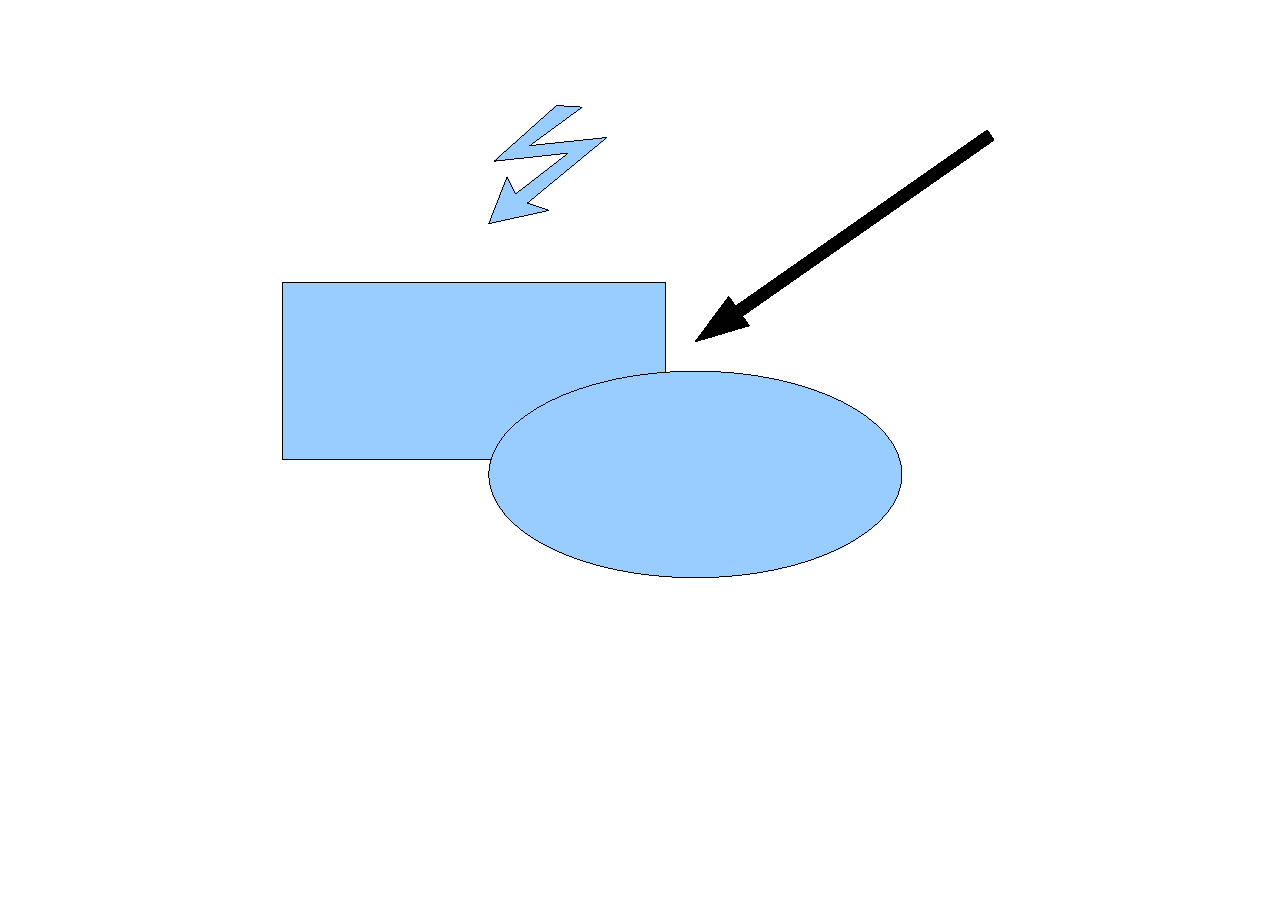
\includegraphics[width=8cm]{Dessin.eps}
\subsection {Mode mathématique}
C'est un des points forts de latex qui permet d'écrire des formules mais aussi des caractères spéciaux tels que :
$2^{32} \approx 10^{9}$ car $\log{_{10}}{2} \approx 0.3$ et $32*0.3 \approx 9$.
\subsection {Quelques trucs faciles}
\begin{itemize}
\item \verb+\\+ permet de passer à la ligne suivante.
\item \verb+\\[2cm]+ permet de passer à la ligne suivante + une tabulation verticale de 2cm. Sont autorisés mm, cm et pts.
\item \verb+\newpage+ permet de forcer un passage à la page suivante.
\end{itemize}
\subsection {Compiler le texte}
Un script permet d'automatiser cette compilation:
\begin{lstlisting}
#! /bin/sh
FN=Mrapport # Le nom du document.
latex $FN.tex
latex $FN.tex # 2 passages pour la TOC
rm $FN.aux $FN.log $FN.out
dvips $FN.dvi -o $FN.ps
rm $FN.dvi
gv $FN.ps # pour visualiser et imprimer
\end{lstlisting}
%-----------------------------------------------------------------------------------
\section{Conclusions}
Ce travail montre, qu'en quelques minutes, on peut déjà fournir un travail présenté de façon professionnelle, lisible par tous et dans un format standard.
Pour ne pas avoir de soucis, les commandes à utiliser pour obtenir un document postcript sont latex et dvips, il ne faut jamais utiliser pdflatex. 

Ce document peut être encore complété avec d'autres exemples qui seraient utiles. Ces nouveaux exemples pourraient être intégrés dans le premier ou un deuxième chapitre. Ceci, sans oublier qu'il s'agit d'un document utile pour commencer très rapidement à écrire en latex et non un mode d'emploi complet de latex qui serait obligatoirement très volumineux.
%-----------------------------------------------------------------------------------
\section{Références}
\begin{itemize}
\item http://www.grappa.univ-lille3.fr/FAQ-LaTeX/ 
\item http://tex.loria.fr/
\item http://tex.loria.fr/english/packages.html
\end{itemize}
%-----------------------------------------------------------------------------------
\section{Annexes }
Vous trouvez dans le casier, un répertoire LATEX contenant :
\begin{itemize}
\item Mrapport.tex : le document latex maître
\item LatexSimple.tex : ce document latex
\item dessin.odg et dessin.eps : le dessin intégré dans le texte
\item go : un script qui permet de compiler rapport.tex, sans argument.
\end{itemize}
%-----------------------------------------------------------------------------------

